%
% main.tex -- Paper zum Thema <wirbelringe>
%
% (c) 2020 Autor, OST Ostschweizer Fachhochschule
%
% !TEX root = ../../buch.tex
% !TEX encoding = UTF-8
% LTeX: enabled=false
\chapter{Wirbelringe\label{chapter:wirbelringe}}
\kopflinks{Wirbelringe}
\begin{refsection}
\chapterauthor{Nino Briker, Fabian Steiner}

% Ein paar Hinweise für die korrekte Formatierung des Textes
% \begin{itemize}
% \item
% Absätze werden gebildet, indem man eine Leerzeile einfügt.
% Die Verwendung von \verb+\\+ ist nur in Tabellen und Arrays gestattet.
% \item
% Die explizite Platzierung von Bildern ist nicht erlaubt, entsprechende
% Optionen werden gelöscht. 
% Verwenden Sie Labels und Verweise, um auf Bilder hinzuweisen.
% \item
% Beginnen Sie jeden Satz auf einer neuen Zeile. 
% Damit ermöglichen Sie dem Versionsverwaltungssysteme, Änderungen
% in verschiedenen Sätzen von verschiedenen Autoren ohne Konflikt 
% anzuwenden.
% \item 
% Bilden Sie auch für Formeln kurze Zeilen, einerseits der besseren
% Übersicht wegen, aber auch um GIT die Arbeit zu erleichtern.
% \end{itemize}

%
% intro.tex -- Einleitung zum Thema
%
% !TEX root = ../../buch.tex
% !TEX encoding = UTF-8
%
\section{Einleitung}

Wirbelringe sind ein interessantes Naturphänomen welchem man schneller begegnet als man denkt. 
In diesem Paper schauen wir uns Wirbelringe etwas genauer an und begründen einige Eigenschaften. 
Des Weiteren untersuchen wir eine weitverbreitete praktische (ungewollte) Anwendung und dessen Auswirkung. 
Zuletzt formulieren wir ein Modell womit man zumindest angenähert selbst gezielt Wirbelringe berechnen und erzeugen kann.

In diesem Paper werden, wo nicht anders angegeben, nur ideale Fluide betrachtet.

\begin{quote}
    The theory of inviscid fluids is the study of «dry water».

    - John von Neumann \cite{Wirbelringe:feynman1964lectures}
\end{quote}

\subsection{Wirbel}

\begin{figure}
\centering
\begin{tikzpicture}
\clip (-6.3,-2.7) rectangle (6.3,2.7);
\node at (-0.07,-0.07) {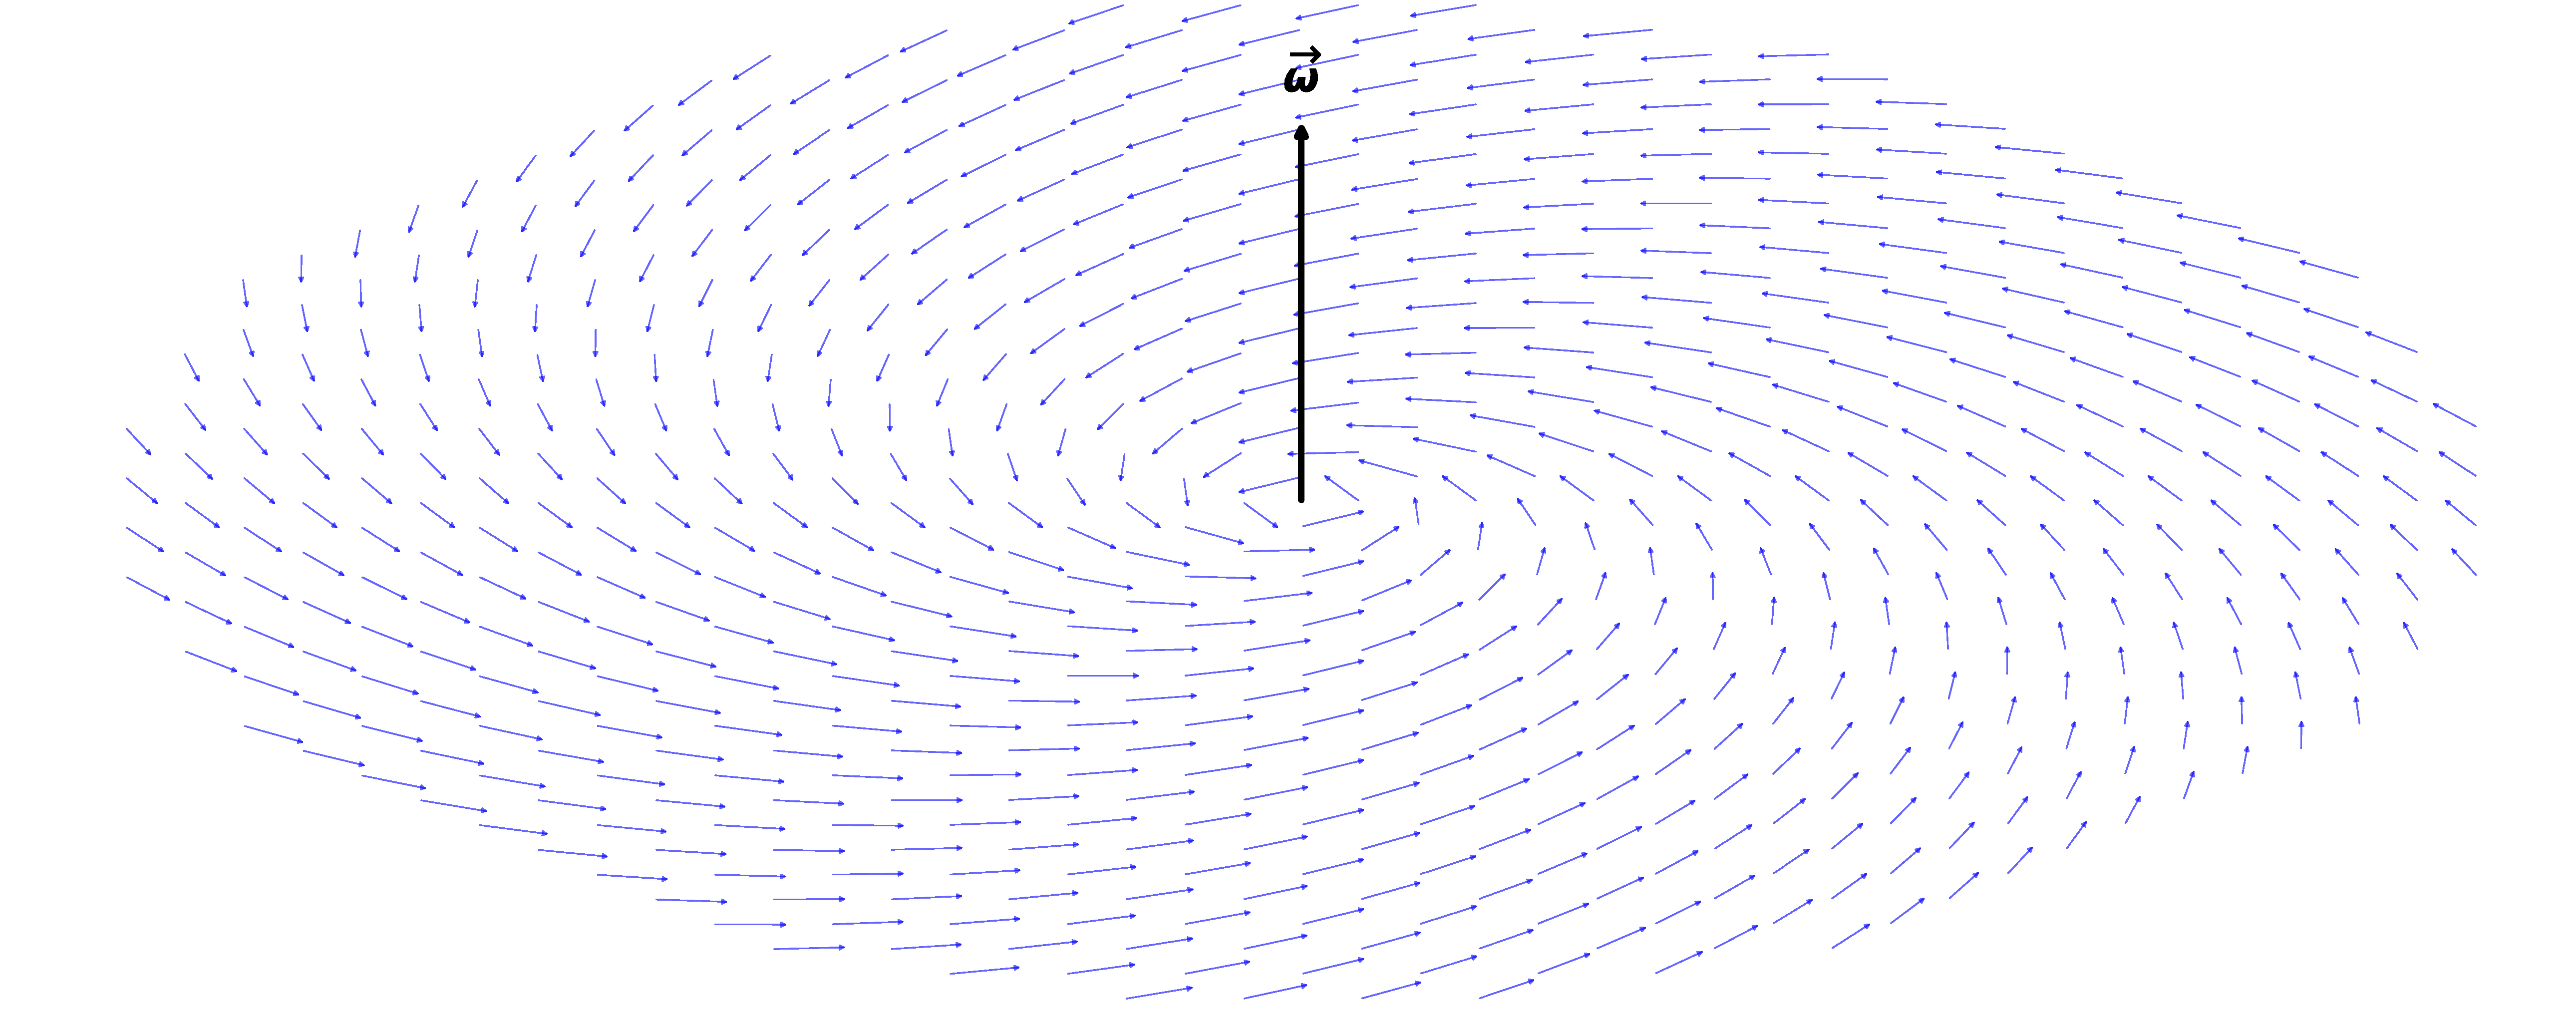
\includegraphics[width=1.08\textwidth]{papers/wirbelringe/fig/flacher_wirbel.pdf}};
%\draw[color=red] (-6.3,-2.7) rectangle (6.3,2.7);
\end{tikzpicture}
\caption{Darstellung eines 2-dimensionalen Wirbels mit Wirbelvektor
\(\vec{\omega}\).
\label{Wirbelringe:fig:flacher_wirbel}}
\end{figure}


Für die Betrachtung von Wirbelringen starten wir zunächst mit einzelnen Wirbeln.
Ein Wirbel ist eine Formation von Teilchen, welche um einen Mittelpunkt rotieren.
In Abbildung \ref{buch:papers:Wirbelringe:fig:flacher_wirbel} ist ein Wirbel abgebildet.
Die eingezeichneten Pfeile stellen die Geschwindigkeitsvektoren \( \vec{v} \) von den Teilchen dar, welche Teil des Wirbels sind.
Nicht explizit eingezeichnet sind die Bahnen, auf welchen sich die Teilchen bewegen.
Die Bahnen bilden konzentrische Kreise.
Auch ist in der Abbildung \ref{buch:papers:Wirbelringe:fig:flacher_wirbel} der Wirbelstärkevektor \(\vec{\omega}\) eingezeichnet.
Wir kommen später genauer auf \(\vec{\omega}\) zu sprechen.

\subsubsection*{Wirbellinien \label{paper:Wirbelringe:Wirbellinien}}

Um Wirbel besser zu beschreiben, führen wir hier den Begriff {\em Wirbellinie} ein.
Wirbellinien sind die „Mittelachsen“ eines Wirbels. 
Um diese Achse rotieren die Teile, welche Teil eines Wirbels sind. 
Diese hat an sich kein Volumen, allerdings kann es sein, dass Teilchen auf dieser Achse zu liegen kommen. 
\(\vec{\omega}\) steht tangential zu dieser Wirbellinie.  
In der Praxis ist eine Wirbellinie nicht gerade, sondern gekrümmt oder sogar spiralenähnlich. 
Des Weiteren ist eine sehr wichtige Eigenschaft, dass Wirbellinien nur auf einer Grenzfläche enden können, 
wie wir in Abschnitt \ref{paper:Wirbelringe:Grenzflaechen} sehen werden.

\subsection{Stabilität}

Um die Stabilität von Wirbeln zu beurteilen, können wir betrachten wie sich die Menge an Teilchen verhaltet, ob sie wächst oder schrumpft. 
Also die Divergenz der Teilchen, die Teil eines Wirbels sind.
Mit dieser Frage kommt man auf die Rechnung
\[
\operatorname{div} ( \operatorname{rot} ( \vec{A} ) )
= % \overset{!}{=}
?,
\]
wobei wir für \(\vec{A}\) das Vektorfeld aus Abbildung \ref{buch:papers:Wirbelringe:fig:flacher_wirbel} verwenden.
Nehmen wir an das \(\vec{A}\) zweimal stetig differenzierbar ist, so erhalten wir
\begin{align*}
\operatorname{div} ( \operatorname{rot} ( \vec{A} ) )
&=
\operatorname{div}      
    \begin{pmatrix} 
        \frac{\partial A_z}{\partial y} - \frac{\partial A_y}{\partial z} \\ 
        \frac{\partial A_x}{\partial z} - \frac{\partial A_z}{\partial x} \\ 
        \frac{\partial A_y}{\partial x} - \frac{\partial A_x}{\partial y} \\ 
    \end{pmatrix} \\
&=
\frac{\partial^2 A_z}{\partial x \partial y} - \frac{\partial^2 A_y}{\partial x \partial z} + 
\frac{\partial^2 A_x}{\partial y \partial z} - \frac{\partial^2 A_z}{\partial y \partial x} +
\frac{\partial^2 A_y}{\partial z \partial x} - \frac{\partial^2 A_x}{\partial z \partial y}
\\
&=
\frac{\partial^2 A_z}{\partial x \partial y} - \frac{\partial^2 A_z}{\partial y \partial x} + 
\frac{\partial^2 A_x}{\partial y \partial z} - \frac{\partial^2 A_x}{\partial z \partial y} +
\frac{\partial^2 A_y}{\partial z \partial x} - \frac{\partial^2 A_y}{\partial x \partial z}
\quad \text{(Satz von Schwarz)}\\
&=
\overbrace{\frac{\partial^2 A_z}{\partial x \partial y} - \frac{\partial^2 A_z}{\partial x \partial y}}^0 + 
\overbrace{\frac{\partial^2 A_x}{\partial y \partial z} - \frac{\partial^2 A_x}{\partial y \partial z}}^0 +
\overbrace{\frac{\partial^2 A_y}{\partial x \partial z} - \frac{\partial^2 A_y}{\partial x \partial z}}^0
\\
&=
0
\end{align*}

Aus dem Resultat
\begin{equation}
    \label{paper:Wirbelringe:eq:wIdent}
\operatorname{div} ( \operatorname{rot} ( \vec{A} ) ) 
= 
0
\end{equation}
lässt sich schliessen, dass Teilchen in einem Rotationsfeld erhalten bleiben. 
Das bedeutet, dass sie immer weiter rotieren. 
Aus diesem Grund sind Wirbel sehr Stabil.

\subsection{Vom Wirbel zum Wirbelring}

Um aus Wirbel ein Wirbelring zu machen brauchen wir noch eine Definition.

\subsubsection*{Wirbelfäden}

Ein {\em Wirbelfaden} ist ein Zylinder, welcher eine Wirbellinie als Zentrum des Zylinders hat.
Schneidet man nun diesen Zylinder senkrecht zu der Wirbellinie, ergibt sich ein einzelner Wirbel.
Wirbelfäden werden auch {\em Wirbelröhren} genannt.

Um aus einem Wirbelfaden ein Wirbelring zu machen, schliessen wir die offenen enden (wir betrachten später, wie man mit diesen umzugehen hat) zusammen.
Die Wirbellinie formt ein Kreis.
Jetzt ist es ein Wirbelring. 
Solch ein Wirbelring ist in Abbildung \ref{buch:papers:Wirbelringe:fig:generell} dargestellt.

\begin{figure}
\centering
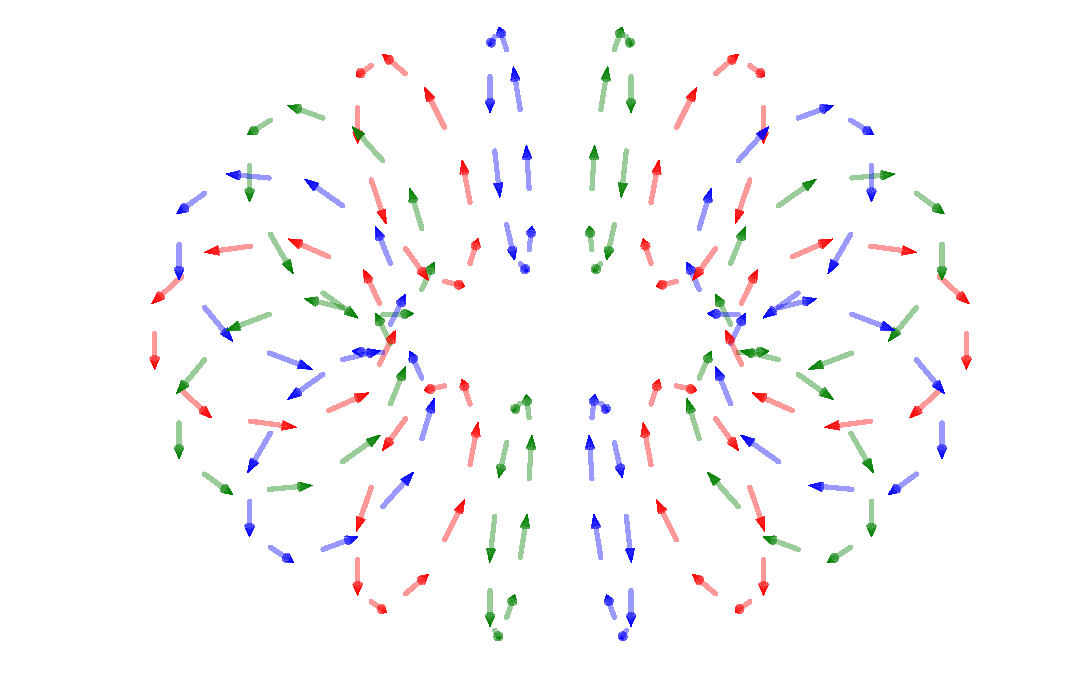
\includegraphics[width=1\textwidth]{papers/wirbelringe/fig/wirbelring_RGB.pdf}
\caption{Typischer idealer Wirbelring.
Dargestellt durch momentane Bewegungsvektoren unterschiedlicher Teilchen in regelmässigem Abstand.
Zur besseren Übersicht sind Teilchen eines Wirbels mit derselben Farbe markiert.
Unterschiedliche, benachbarte Wirbel haben unterschiedliche Farben.
Die Wirbellinie ist als schwarze, gestrichelte Linie eingezeichnet.\label{Wirbelringe:fig:generell}}
\end{figure}

\section{Helmholzsche Wirbelsätze}

\subsection{Historisches}

Um das Verhalten von Wirbelringen besser zu verstehen, sind die sogenannten helmholzschen Wirbelsätze sehr nützlich. 
Mitte 19. Jahrhundert formulierte der Deutsche Physiker Hermann von Helmholtz 3 Wirbelsätze und veröffentlichte diese im Journal für die reine und angewandte Mathematik\cite{Wirbelringe:JournalHelmholz}.
In dieser definiert er auch gleich auch Hilfslinien, um die Wirbelbewegungen, besser beschreiben zu können:

\subsubsection*{Wirbellinien}

Wirbellinien sind die „Mittelachse“ eines Wirbels. 
Um diese Achse rotieren die Teile, welche teil eines Wirbels sind. 
Diese hat an sich kein Volumen, allerdings kann es sein das Teilchen auf dieser Achse zu liegen kommen. 

\subsubsection*{Wirbelfäden}



\subsection{Erster Helmholzscher Wirbelsatz}

\begin{displayquote}
    In Abwesenheit von wirbel anfachenden äusseren Kräften bleiben wirbelfreie Strömungsgebiete wirbelfrei.
\end{displayquote}

Teilchen die, ruhen bleiben in ruhe.

\begin{figure}
\centering
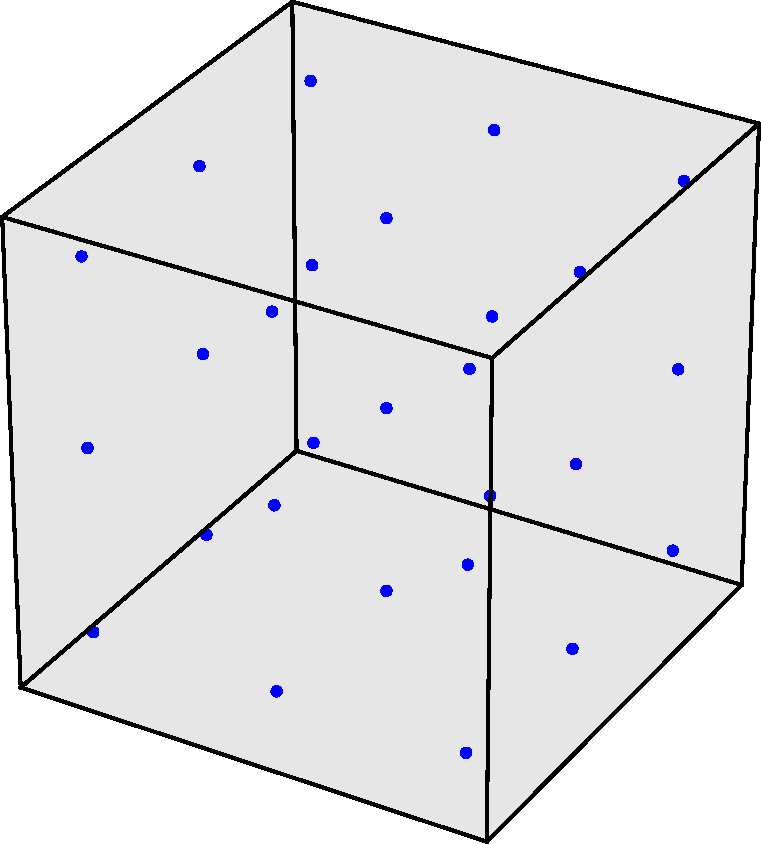
\includegraphics[width=0.4\textwidth]{papers/wirbelringe/fig/cube_still_particles.pdf}
\caption{Visuelle Darstellung des 1. helmholtzschen Wirbelsatz \label{buch:papers:Wirbelringe:fig:Helmholtz_1}}
\end{figure}

\subsection{Zweiter Helmholzscher Wirbelsatz}

\begin{displayquote}
    Fluidelemente, die auf einer Wirbellinie liegen, verbleiben auf dieser Wirbellinie.
\end{displayquote}

\begin{figure}
\centering
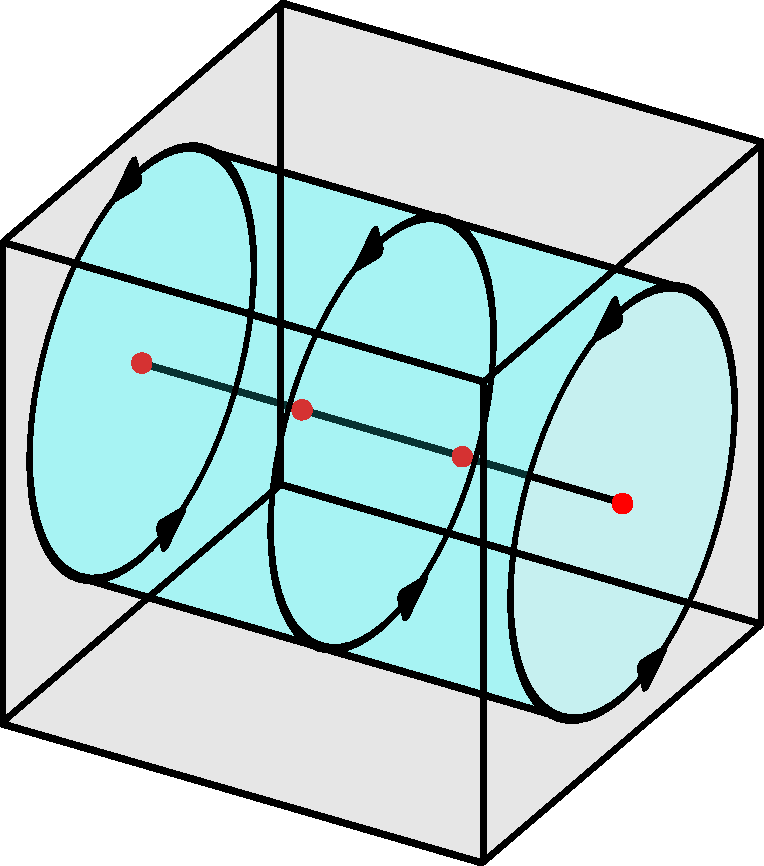
\includegraphics[width=0.4\textwidth]{papers/wirbelringe/fig/cube_still_particles_rotation.pdf}
\caption{Visuelle Darstellung des 2. helmholtzschen Wirbelsatz \label{buch:papers:Wirbelringe:fig:Helmholtz_2}}
\end{figure}

\subsection{Dritter Helmholzscher Wirbelsatz}

\begin{displayquote}
    Fluidelemente, die auf einer Wirbellinie liegen, verbleiben auf dieser Wirbellinie.
\end{displayquote}

\begin{figure}
\centering
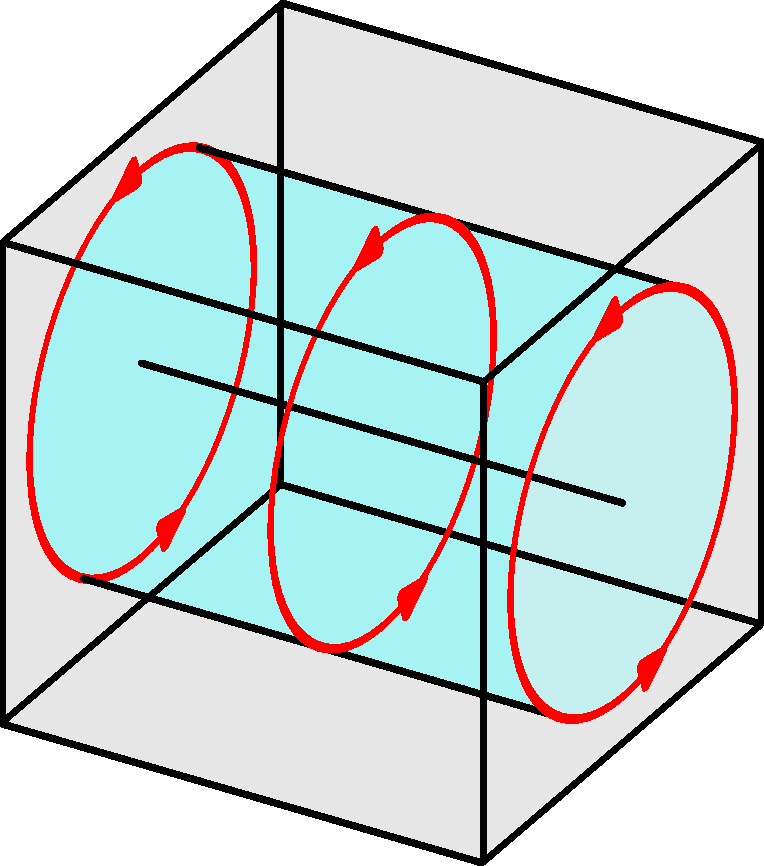
\includegraphics[width=0.4\textwidth]{papers/wirbelringe/fig/cube_constant_rotation.pdf}
\caption{Visuelle Darstellung des 3. helmholtzschen Wirbelsatz \label{buch:papers:Wirbelringe:fig:Helmholtz_3}}
\end{figure}

\subsection{Verhalten an Grenzflächen}

\printbibliography[heading=subbibliography]
\end{refsection}
